\documentclass[letter]{article}
\usepackage[cm]{fullpage}
\usepackage[table]{xcolor}
\usepackage{listings}
\usepackage{graphicx}
\usepackage{hyperref}
%package below is for adding images in exact place in code
\usepackage{float}
\usepackage[toc,page]{appendix}

 
\setlength{\arrayrulewidth}{1mm}
\setlength{\tabcolsep}{18pt}
\renewcommand{\arraystretch}{2.5}

\graphicspath{ {images/} }

%background color for source code snippets and links 
\definecolor{mygray}{gray}{0.95}

%for changing color in links
\hypersetup{
    colorlinks,
    linkcolor={black},
    citecolor={blue!50!black},
    urlcolor={blue!80!black}
}

%source code with highliting
\lstset{basicstyle=\fontsize{9}{10}\ttfamily,
	backgroundcolor=\color{mygray},
  	%commentstyle=\color{blue},
  	%keywordstyle=\color{blue}
	language=bash,
	xleftmargin=\parindent,
	extendedchars=true, 
	showspaces=false,
	showstringspaces=false,
}

%for an src directory of bash scripts
\newcommand*\lstinputpath[1]{\lstset{inputpath=#1}}
\lstinputpath{src}

%prints out helpful info with layout uncommented below
%\usepackage{layout}

\title{Performance Analysis on Intel XL710 using DPDK i40e Poll Mode Driver \\ Tests on ppc64le using DPDK v17.11}
\author{Mick Tarsel \\  LTC Networking Team \\}  

\begin{document}
%\layout

\maketitle

\newpage
\tableofcontents
\newpage

\section{Machine Information}

The purpose of this test plan is to test Open vSwitch (OvS). 
The document provides commands and the expected output.
This test plan aims to provide a pass/failure reference point based on the output of the command.
Output may change over time due to the nature of this project, however certain information should still be retained from output to signify a pass or failure.
Important information from output will be \setlength{\fboxsep}{0pt}\colorbox{yellow}{{\textcolor{red}{highlited}}}. 
Verify that your output has something similar to the highlited parts of the output.

Each section is self-containing such that you may skip around the document.
After setup and execution of tests, the test concludes with a verification section. 
Highlited output missing from verification section would indicate a failure.
If there is a possibility of a failure refer to the Appendix first.
Make sure you remove previous bridges or interfaces before moving to the next test in case there is a naming conflict.

This test plan utilizes network name spaces (ns) to create virtual network endpoints in order to test the features of OvS. 
Each network name space will be an endpoint on our virtual switch. 
The picture below represents the basic network topology this test plan will use. 

Looking at the diagram above we see 3 name spaces. One root name space, and 2 network name spaces. The veth peers for \texttt{namespace1} are \texttt{tap1} and \texttt{p1}. \texttt{tap1} device exists only inside namespace1. Much similar to a VM having a different Ethernet interface than the host machine. \textit{Please note that root namespace and host are used interchanbly throughout the document.} \texttt{p1} exists on the host and in this picture it has been added as a port to the OvS bridge named \texttt{br-1}. Additional information about name spaces may be found in appendix \ref{appendix:ns}.

Commands below are going to be used most often in this test plan
\begin{itemize}
\item \texttt{ovs-vsctl} : Used for configuring the ovs-vswitchd configuration database (known as ovs-db) 
\item \texttt{ovs-ofctl} : A command line tool for monitoring and administering OpenFlow switches 
%The follow are not used yet
%\item \texttt{ovs-dpctl} : Used to administer Open vSwitch datapaths
\item \texttt{ovs-appctl} : A utility that sends commands to and controls Open vSwitch daemons 
\item \texttt{ovsdb-tool} : Open vSwitch database management utility
\item \texttt{netperf} : a network performance benchmark
\item \texttt{tcpdump} : dump traffic on a network
\item \texttt{netcat} : create, concatenate, and redirect sockets. 
%\item \texttt{ovsdb-server} : TODO
%\item \texttt{ip addr} :  show or manipulate routing, devices, policy routing and tunnels
%\item \texttt{ip netns exec} : process network namespace management
%\item \texttt{modprobe} : Add or remove modules from Linux kernel
%\item \texttt{modinfo} : Show information about a Linux kernel module
%\item \texttt{ps} : Report a snapshot of the current processes
\end{itemize}

Any refernce to another section will be a clickable link to that section.

%%%%%%%%%%%%%%%%%%%%%%%%%%%%%%%%%%%%%%%%%%%%%%%%%%%%%
%%%  RX only bandwidth using testpmd
%%%%%%%%%%%%%%%%%%%%%%%%%%%%%%%%%%%%%%%%%%%%%%%%%%%%%

\section{RX Only Bandwidth using testpmd}
%to many 1 line explanations that should not be indented.
{\setlength{\parindent}{0cm}

\begin{figure}[H]
\caption{some caption}
\hbox{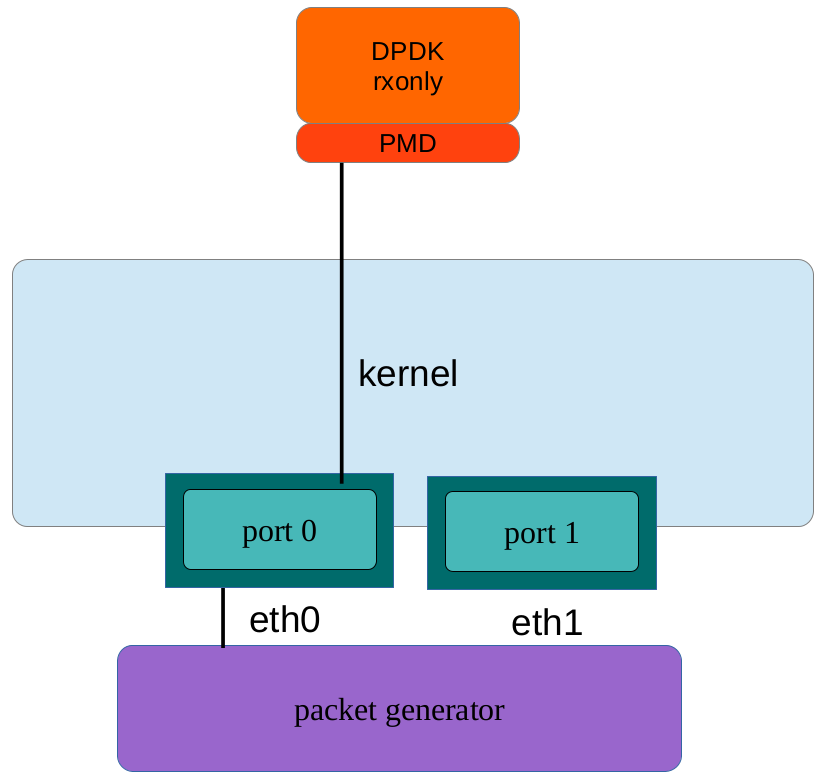
\includegraphics[scale=0.6]{rx-only} }
\end{figure}

\rowcolors{3}{green!80!yellow!50}{green!70!yellow!40}
\begin{tabular}{ |p{3cm}|p{3cm}|p{3cm}|  }
\hline
\multicolumn{3}{|c|}{Country List} \\
\hline
Country Name     or Area Name& ISO ALPHA 2 Code &ISO ALPHA 3 \\
\hline
Afghanistan & AF &AFG \\
Aland Islands & AX   & ALA \\
Albania &AL & ALB \\
Algeria    &DZ & DZA \\
American Samoa & AS & ASM \\
Andorra & AD & AND   \\
Angola & AO & AGO \\
\hline
\end{tabular}

\begin{center}
\begin{tabular}{ |c|c|c| } 
 \hline
 cell1 & cell2 & cell3 \\ 
 cell4 & cell5 & cell6 \\ 
 cell7 & cell8 & cell9 \\ 
 \hline
\end{tabular}
\end{center}



\subsection{pktgen Machine (126)}

% ./pktgen -l 0-3,8-11,16-19,24-27,32-35,40-43,48-51,56-59,64-67,72-75 --socket-mem=4096,4096 -- -T -P -m "[8:40-43/48-51].0"
\begin{lstlisting}
pktgen -l 0-3,8-11,16-19,24-27,32-35,40-43,48-51,56-59,64-67,72-75 --socket-mem=4096,4096 
	-- -T -P -m "[8:40-43/48-51].0"
\end{lstlisting}

\subsection{testpmd (124)}

% Q=8; testpmd -l 0,8,16,24,32,40,48,56,64,72 -m 4096 -w 0002:01:00.0 -- --txd=512 --rxd=512 --mbcache=512 --rxq=$Q--txq=$Q --nb-cores=$Q -i -a --rss-ip --forward-mode=rxonly  --port-topology=chained
\begin{lstlisting}[escapechar=!]
Q=8; testpmd -l 0,8,16,24,32,40,48,56,64,72 -m 4096 -w 0002:01:00.0 
-- --txd=512 --rxd=512 --mbcache=512 --rxq=$Q--txq=$Q --nb-cores=$Q -i -a 
	--rss-ip --forward-mode=rxonly  --port-topology=chained
\end{lstlisting}

\subsection{Starting Test}

\begin{lstlisting}[escapechar=!]
Pktgen:/> start 0
\end{lstlisting}

\begin{lstlisting}
testpmd> show port stats all

  ######################## NIC statistics for port 0  ########################
  RX-packets: 16519665   RX-missed: 48236188   RX-bytes:  3885350400
  RX-errors: 0
  RX-nombuf:  0         
  TX-packets: 16         TX-errors: 0          TX-bytes:  0

  Throughput (since last show)
  Rx-pps:     24898418
  Tx-pps:            0
  ############################################################################
testpmd> 
\end{lstlisting}

%%%%%%%%%%%%%%%%%%%%%%%%%%%%%%%%%%%%%%%%%%%%%%%%%%%%%
%%% I/O forward across 2 ports
%%%%%%%%%%%%%%%%%%%%%%%%%%%%%%%%%%%%%%%%%%%%%%%%%%%%%
\section{I/O forward bandwidth using testpmd across ports}
%to many 1 line explanations that should not be indented.
{\setlength{\parindent}{0cm}

\begin{figure}[H]
\caption{Path of ICMP packet from \texttt{namespace1} through \texttt{br-1} to \texttt{namespace2}}
\hbox{\hspace{-0.5cm} 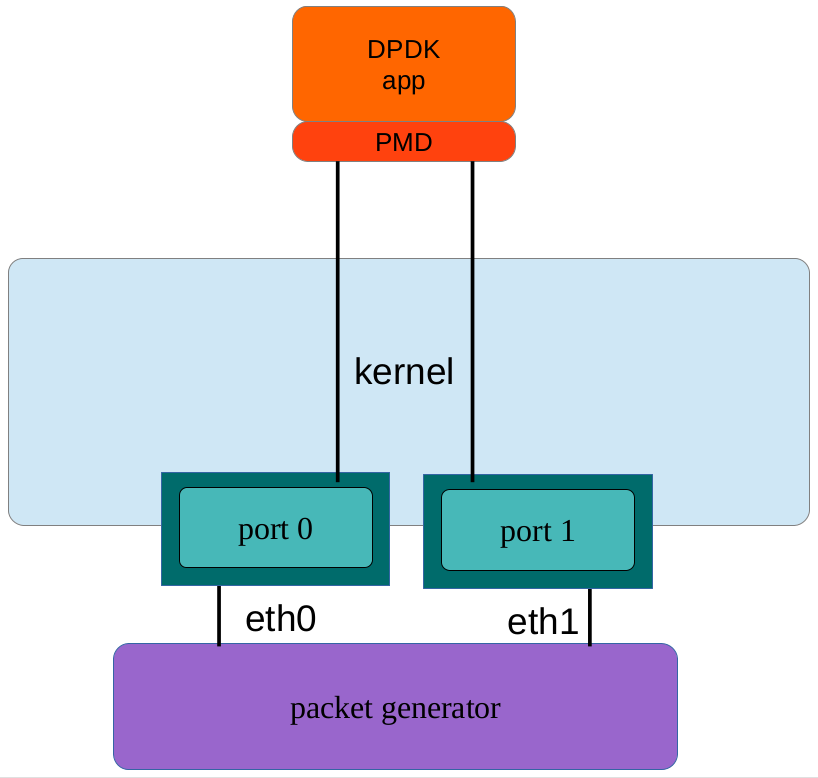
\includegraphics[scale=0.6]{i-o-2-ports} }
\end{figure}

\subsection{pktgen Machine (126)}

% ./pktgen -l 0-3,8-11,16-19,24-27,32-35,40-43,48-51,56-59,64-67,72-75 --socket-mem=4096,4096 -- -T -P -m "[8:40-43/48-51].0,[56-59/64-67:72].1"
\begin{lstlisting}
pktgen -l 0-3,8-11,16-19,24-27,32-35,40-43,48-51,56-59,64-67,72-75 --socket-mem=4096,4096 
	-- -T -P -m "[8:40-43/48-51].0,[56-59/64-67:72].1"
\end{lstlisting}

\subsection{testpmd (124)}

% testpmd -l 0,8,16,24,32,40,48,56,64,72 -m 4096 -w 0002:01:00.0 -w 0002:01:00.1 -- --txd=512 --rxd=512 --mbcache=512 --rxq=$Q --txq=$Q --nb-cores=$Q -i -a --rss-ip --forward-mode=io
\begin{lstlisting}[escapechar=!]
testpmd -l 0,8,16,24,32,40,48,56,64,72 -m 4096 -w 0002:01:00.0 -w 0002:01:00.1 -- --txd=512
--rxd=512 --mbcache=512 --rxq=$Q --txq=$Q --nb-cores=$Q -i -a --rss-ip --forward-mode=io
\end{lstlisting}

\subsection{Starting Test}

\begin{lstlisting}[escapechar=!]
Pktgen:/> enable 0 range
-- Pktgen 
Pktgen:/> start 0
\end{lstlisting}

\begin{lstlisting}
Port 0: LSC event
Port 1: LSC event
testpmd> show port stats all
testpmd> show port stats all

  ######################## NIC statistics for port 0  ########################
  RX-packets: 15107923   RX-missed: 62402292   RX-bytes:  4650612480
  RX-errors: 0
  RX-nombuf:  0         
  TX-packets: 30         TX-errors: 0          TX-bytes:  1440

  Throughput (since last show)
  Rx-pps:     20292924
  Tx-pps:            5
  ############################################################################

  ######################## NIC statistics for port 1  ########################
  RX-packets: 30         RX-missed: 0          RX-bytes:  1440
  RX-errors: 0
  RX-nombuf:  0         
  TX-packets: 15108497   TX-errors: 0          TX-bytes:  906509264

  Throughput (since last show)
  Rx-pps:            5
  Tx-pps:     20292567
  ############################################################################
testpmd> 

\end{lstlisting}

%%%%%%%%%%%%%%%%%%%%%%%%%%%%%%%%%%%%%%%%%%%%%%%%%%%%%
%%% I/O forward across 1 port
%%%%%%%%%%%%%%%%%%%%%%%%%%%%%%%%%%%%%%%%%%%%%%%%%%%%%
\section{I/O forward bandwidth using testpmd within same port}
%to many 1 line explanations that should not be indented.
{\setlength{\parindent}{0cm}

\begin{figure}[H]
\caption{Path of ICMP packet from \texttt{namespace1} through \texttt{br-1} to \texttt{namespace2}}
\hbox{\hspace{-0.5cm} 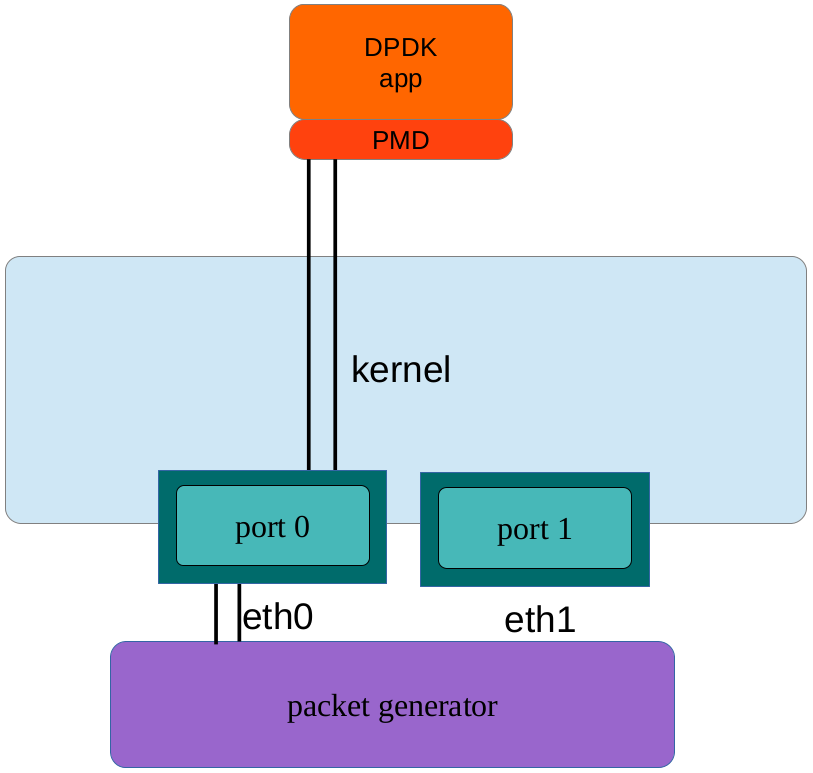
\includegraphics[scale=0.6]{i-o-1-port} }
\end{figure}

\subsection{pktgen Machine (126)}

% ./pktgen -l 0-3,8-11,16-19,24-27,32-35,40-43,48-51,56-59,64-67,72-75 --socket-mem=4096,4096 -- -T -P -m "[8-11/16-19:40-43/48-51].0"
\begin{lstlisting}
# pktgen -l 0-3,8-11,16-19,24-27,32-35,40-43,48-51,56-59,64-67,72-75 
	--socket-mem=4096,4096 -- -T -P -m "[8-11/16-19:40-43/48-51].0"
\end{lstlisting}

\subsection{testpmd (124)}

% testpmd -l 0,8,16,24,32,40,48,56,64,72 -m 4096 -w 0002:01:00.0 -- --txd=512 --rxd=1024 --mbcache=512 --rxq=$Q --txq=$Q --nb-cores=$Q -i -a --rss-ip --forward-mode=io 
\begin{lstlisting}[escapechar=!]
# testpmd -l 0,8,16,24,32,40,48,56,64,72 -m 4096 -w 0002:01:00.0 -- --txd=512 
--rxd=512 --mbcache=512 --rxq=$Q --txq=$Q --nb-cores=$Q -i -a --rss-ip --forward-mode=io
\end{lstlisting}

\subsection{Starting Test}

\begin{lstlisting}[escapechar=!]
Pktgen:/> enable 0 range
-- Pktgen 
Pktgen:/> start 0
\end{lstlisting}

\begin{lstlisting}
Port 0: LSC event
testpmd> show port stats all

  ######################## NIC statistics for port 0  ########################
  RX-packets: 27704184   RX-missed: 42793993   RX-bytes:  4229888660
  RX-errors: 0
  RX-nombuf:  0         
  TX-packets: 27704037   TX-errors: 0          TX-bytes:  1662241920

  Throughput (since last show)
  Rx-pps:     23247541
  Tx-pps:     23247573
  ############################################################################
testpmd>
\end{lstlisting}

}%for no indents on one-liners

\end{document}

